\section{Testing}
Software testing is a process of executing a program or application with the intent of finding the software bugs. It can also be stated as the process of validating and verifying that a software program or application or product: Meets the business and technical requirements that guided it's design and development.

Test Suit for thepoet.me is developed using following two software:

\begin{enumerate}
    \item \textbf{dareboost:} One tool to test, analyze and monitor
    speed and user experience of web pages. Figure \ref{dare}
     \begin{figure}
         \centering
         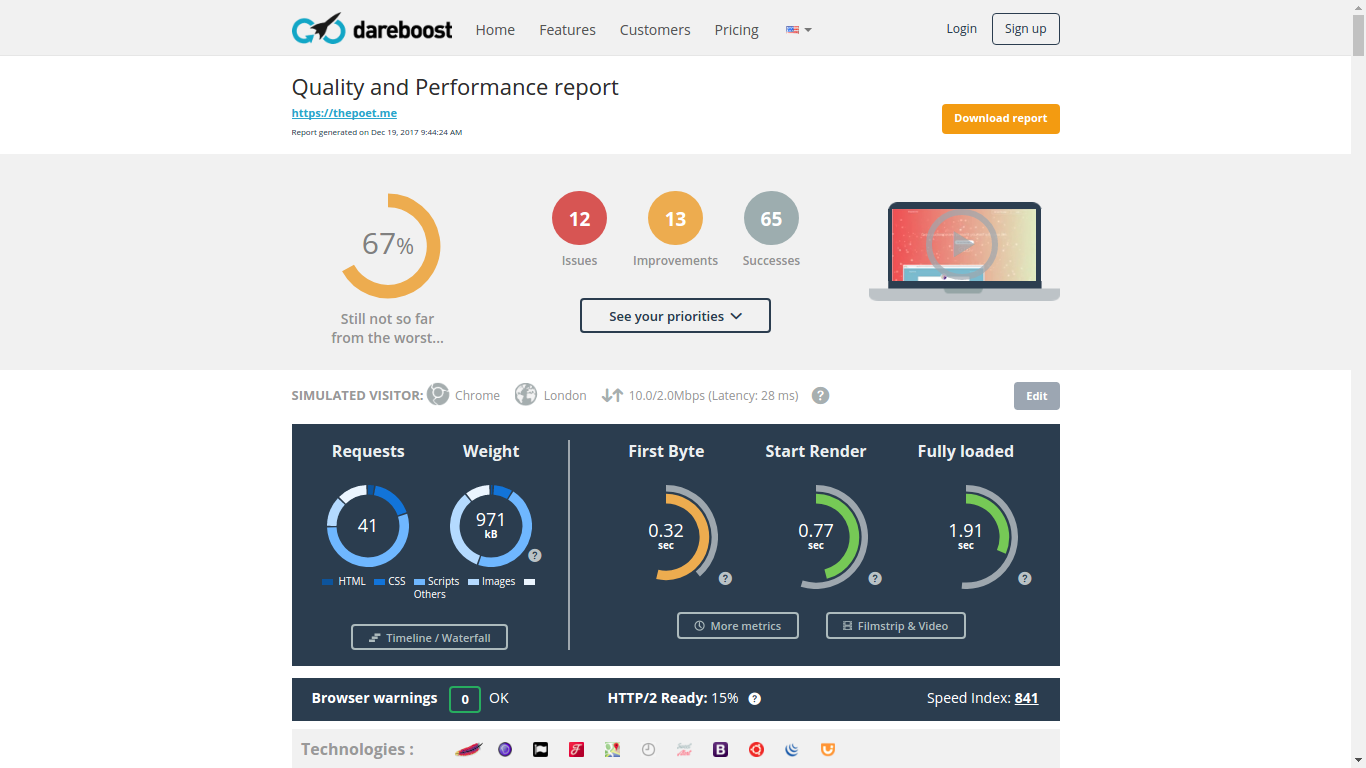
\includegraphics[width=\linewidth]{images/dareboost.png}
         \caption{Performance report by dareboost}
         \label{dare}
     \end{figure}

    \item \textbf{SEO Tool:} A good search engine optimization strategy is based on careful planning, a lot of work and good choices made on key issues. Everything will get analyzed at the end of each month, when the time comes to send out monthly reports to your customers. Figure \ref{dare1}
     \begin{figure}
         \centering
         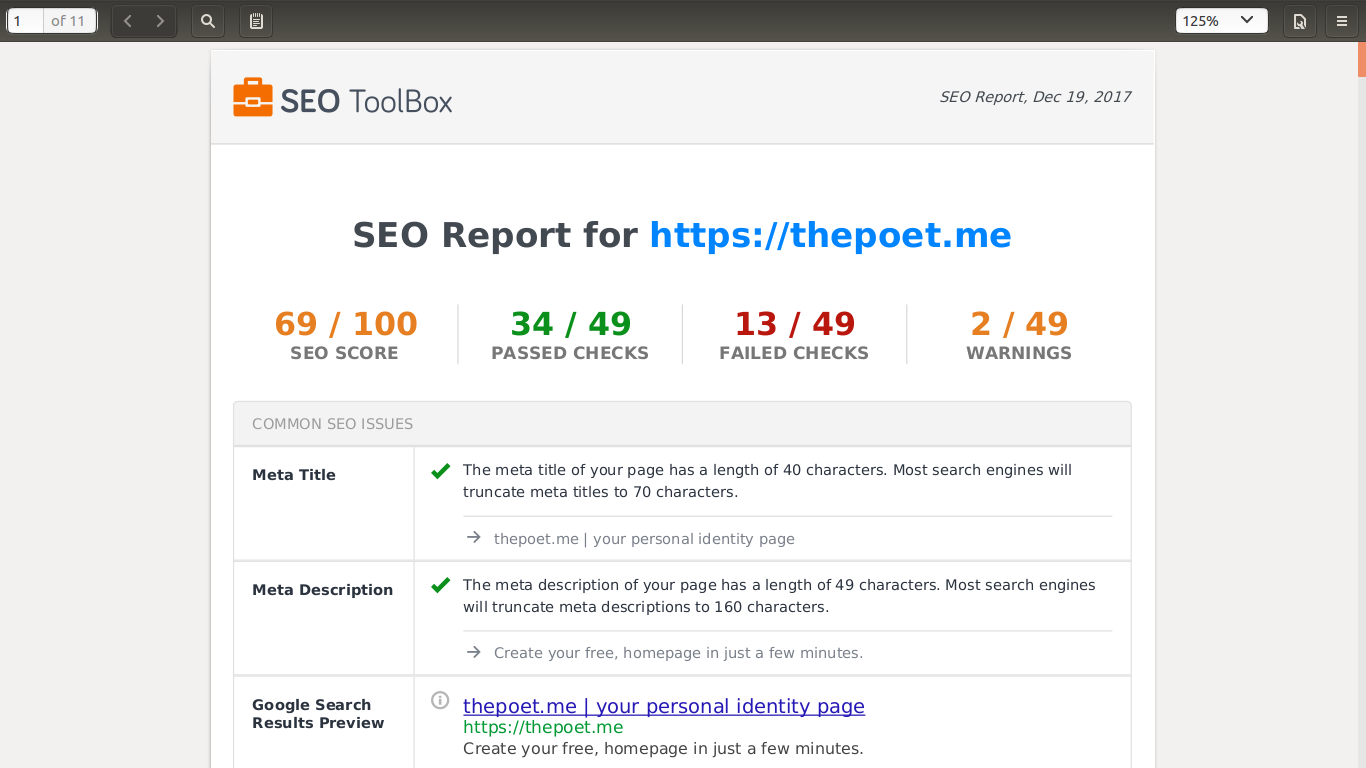
\includegraphics[width=\linewidth]{images/seotool.png}
         \caption{SEO report}
         \label{dare1}
     \end{figure}

\end{enumerate}



%\begin{sidewaystable}
%	\centering
%	\caption{Table to show various Tests}
%	 \begin{tabular}{ |c|c|c|c|c| }
%			\hline
%			\multicolumn{5}{|c|}{Test cases for customizer } \\
%			\hline
%			Sr. & Test Name & Test Description &No. of test Cases& Status \\ \hline
%			1 &customizertest\_description& Check if description syntax work& 24 &Pass\\ \hline
%			2 &customizertest\_parameter& Check if parameter syntax work& 33 &Pass\\ \hline
%			3 &customizertest\_allmodulescomment& Check iteraction of new syntax with modules & 39 &Pass\\ \hline
%			4 &customizertest\_allfunctionscomment & Check iteraction of new syntax with functionas&33 &Pass\\ \hline
%			5 &customizertest\_allexpressionscomment&Check iteraction of new syntax with expressions& 37&Pass\\ \hline
%			6 &customizertest\_group&  Check if group syntax work&16 & Pass\\ \hline
%			7 &customizertest-first\_setofparameter& Check if Json is read correctly& 1& Pass\\ \hline
%			8 &customizertest-wrong\_setofparameter&Check if Json is read correctly for wrong syntax& 1&Pass\\ \hline
%			9 &customizertest-incomplete\_setofparameter& Check if Json is read correctly for incomplete parameters& 1& Pass\\ \hline
%			10 &customizertest-imgset\_setofparameter&Check if Json is read correctly for imaginary set&1 & Pass\\ \hline	
%		\end{tabular}
%	\end{sidewaystable}
		
		
